\begin{figure}
	\tikzsetnextfilename{nastro-moebius}
	\centering
	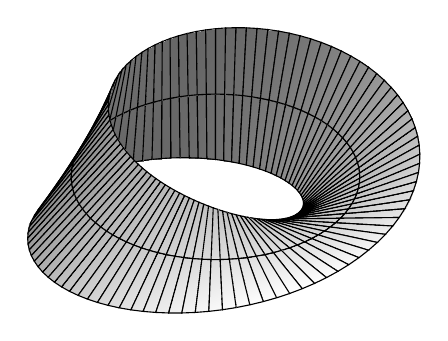
\begin{tikzpicture}
		\begin{axis}[
			trig format plots=rad, % Imposta gli angoli in radianti (dovrebbe esserci un'impostazione globale...) 
			unit vector ratio=1 1 1, % Rapporti tra le lunghezze nelle tre direzioni
			hide axis, % Tengo nascosti gli assi perche' servono a poco in questo caso
			view={70}{35} % {angolo azimutale}{elevazione, attorno all'asse x ruotato}, in gradi/360
			% Con un'elevazione < 30 il nastro appare troppo schiacciato
			% Ho trovato una buona combinazione con un po' di pazienza ;-)
			]
			\addplot3[
				surf,
				faceted color=black,
				shader=faceted interp, % Determina la colorazione della superficie:
				% 'faceted interp' determina il colore di ogni "frammento" della figura
				% con un algoritmo di interpolazione e colora il contorno di ciascuno di essi
				% con il valore assegnato a 'faceted color' precedentemente
				point meta=x, % Per basare la colorazione della superficie sul valore di x
				colormap={bw}{gray(0cm)=(0.4); gray(1cm)=(1)}, % Una colorazione da grigio a bianco
				samples=100,
				samples y=3, % Questo disegna tre righe ``orizzontali'', una in mezzo e due al bordo
				z buffer=sort, % Determina quali parti dell'immagine devono essere disegnate per prime: 'sort'
				% lo decide in modo intelligente, in base alla profondità dei punti
				domain=0:6.284, % x è l'angolo, che va da 0 a poco più di 2pi
				y domain=-1:1 % y è l'altezza del nastro (con questo intervallo è alto 1)
			] (
				{(1+y/2*cos(x/2))*cos(x)},
				{(1+y/2*cos(x/2))*sin(x)},
				{y/2*sin(x/2)}
			);
		\end{axis}
	\end{tikzpicture}
	\caption{Un esempio di nastro di M\"obius, ottenuto dalla \eqref{eq:nastro-moebius} con $r=1$ e $a=1$. Percorrendo la circonferenza al centro del nastro si può notare che fissato localmente un versore normale e prolungandolo per continuità su tutto il nastro, compiendo un giro di $2\pi$ il versore normale risulta orientato nel verso opposto.}
	\label{fig:nastro-moebius}
\end{figure}
